\lstset{  % TODO: trouver comment fix le margin des cellules de codes dans les enum de façon plus propre.
	language=bash,
	basicstyle=\ttfamily,
}

\chapter{Introduction}
\section{L'histoire du C++}

\begin{figure}[ht]
	\centering
	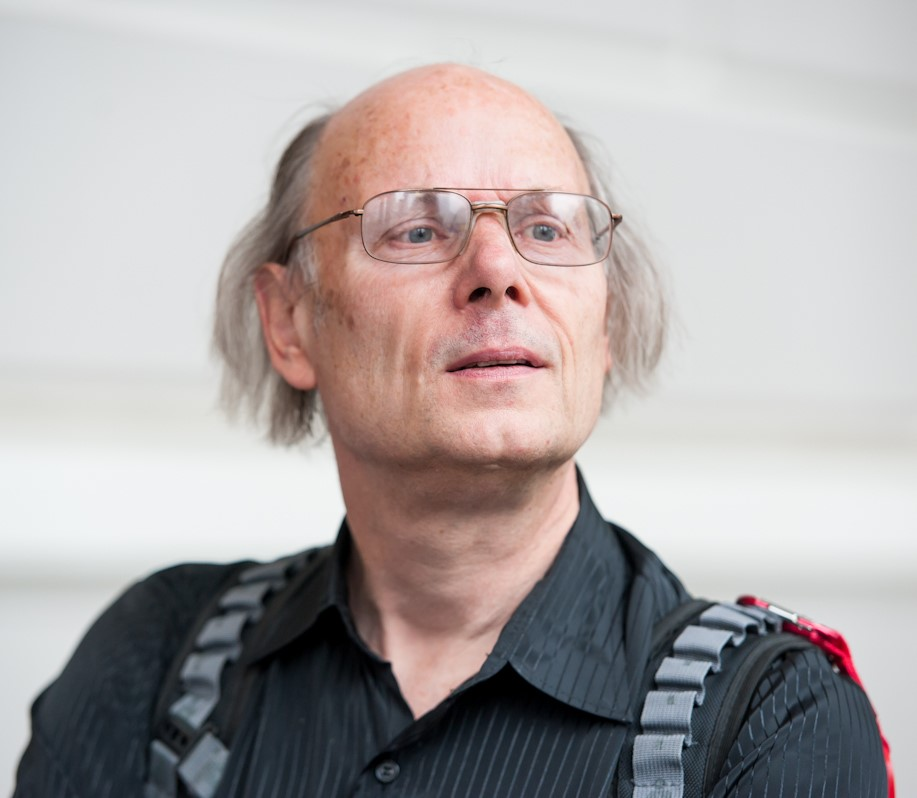
\includegraphics{Images/bjarne_stroustrup}
	\caption{Bjarne Stroustrup (2013)}()
	\label{bjarne_stroustrup}
\end{figure}

Le langage \cpp a été conçu au début des années 1980 par Bjarne Stroustrup (figure~\ref{bjarne_stroustrup}), un ingénieur d'origine danoise, alors qu'il travaillait au sein des laboratoires Bell Labs, un centre de recherche réputé pour ses innovations. Stroustrup souhaitait améliorer le langage C en y intégrant des fonctionnalités de programmation orientée objet, qui permettent de structurer le code de manière plus modulaire et intuitive, notamment grâce à des concepts tels que les classes et les objets. L'objectif principal était de combiner la puissance, la flexibilité et l'efficacité du C avec une organisation et une maintenabilité accrues, afin de faciliter l'écriture et la gestion de programmes complexes. Aujourd'hui, le \cpp demeure l'un des langages de programmation les plus populaires et polyvalents, largement utilisé dans le développement de logiciels, de jeux vidéo, d'applications haute performance, ainsi que dans les systèmes embarqués et d'autres domaines technologiques avancés.

\section{Différences entre C et C++}
Le C et le \cpp sont des langages de programmation étroitement liés, mais ils diffèrent par leurs caractéristiques et leurs usages. Le C est un langage procédural qui se concentre sur les fonctions et les structures de données, idéal pour les systèmes bas-niveau comme les systèmes d'exploitation. En revanche, le \cpp étend le C en introduisant la programmation orientée objet, avec des concepts comme les classes, l'héritage et le polymorphisme, ce qui le rend plus adapté à des projets complexes nécessitant une organisation modulaire. De plus, le \cpp offre des fonctionnalités modernes comme les templates, les exceptions et la gestion automatique des ressources, absentes en C. Malgré leurs différences, \emph{le \cpp reste compatible avec le C}, permettant d'utiliser du code C dans des projets \cpp.

\section{Installation de l'environnement de développement}
Afin d'écrire, compiler et exécuter du code \cpp sur notre machine il est nécessaire d'installer deux outils essentiels: un éditeur de texte et un compilateur. Nous ne verrons pas l'installation de l'éditeur de texte dans ce cours il vous suffit de vous rendre sur le site de votre éditeur de texte de préférence, de télécharger le wizard d'installation correspondant à votre système et de suivre les indications pour pouvoir l'utiliser sur votre machine. Ces éditeurs incluent (mais ne se limitent pas à):

\begin{itemize}
	\item \href{https://code.visualstudio.com/Download}{Visual Studio Code}
	\item \href{https://notepad-plus-plus.org/downloads/v8.7.4/}{Notepad++}
	\item \href{https://www.sublimetext.com/download}{Sublime Text}
\end{itemize}

Concentrons nous donc sur l'installation du compilateur. Pour les utilisateurs de Mac, MacOs possède déjà un compilateur intégré, nous ne nous soucierons donc que des installations sur Windows et Linux.

\subsection{Windows}
\begin{enumerate}
	\item Tout d'abord, rendez vous sur le site de \href{https://www.msys2.org/docs/installer/}{MSYS2} et téléchargez l'installateur.
	\item Lancez l'installateur et suivez les étapes.
	\item Dans l'installateur, choisissez votre dossier d'installation, gardez le en mémoire pour plus tard. Dans la plus part des cas le dossier de base est acceptable.
	\item Une fois l'installation terminée assurez vous que le choix \emph{Run MSYS2 now} est coché puis sélectionnez \emph{Finish}. Cela vous ouvrira un terminal MSYS2.
	\item Dans ce terminal, installez les outils de compilation de MinGW en lançant la commande suivante:
		\begin{lstlisting}[xleftmargin=-12em]
			pacman -S --needed base-devel mingw-w64-ucrt-x86_64-toolchain
		\end{lstlisting}
	\item Acceptez l'installation des packets en pressant la touche "Entrée".
	\item Entrez 'Y' quand le programme vous demande si vous voulez poursuivre l'installation.
	\item Ajoutez le chemin du dossier \emph{bin} de votre installation de MinGW au PATH.
		\begin{enumerate}
			\item Dans la barre de recherche Windows, cherchez \emph{Modifier les variables d'environnement système}.
			\item Dans vos variables d'utilisateur, sélectionnez la variable \emph{Path} et cliquez sur \emph{Modifier}.
			\item Sélectionnez \emph{Nouveau} et ajoutez le chemin du dossier bin. Si vous n'avez pas changé l'adresse de celui proposé lors de l'installation le chemin devrait être le suivant: \emph{C:$\backslash$msys64$\backslash$ucrt64$\backslash$bin}.
			\item Sélectionnez \emph{OK} deux fois.
		\end{enumerate}
	\item Pour vérifier votre installation ouvrez un nouvel invite de commande puis tapez la commande suivante:
		\begin{lstlisting}[xleftmargin=-12em]
			g++ --version
		\end{lstlisting}
		Si vous n'obtenez pas d'erreur alors félicitations ! Vous pouvez désormais compiler du code \cpp !
\end{enumerate}


\subsection{Linux}
Dans un premier temps, mettez à jour votre installateur en exécutant la commande suivante:
\begin{lstlisting}
	sudo apt update
\end{lstlisting}
Ensuite, installez l'outil de compilation \emph{g++} grâce à cette autre commande:
\begin{lstlisting}
	sudo apt install g++
\end{lstlisting}


\subsection{MacOS}
Il est probable que le compilateur \emph{g++} soit déjà installé sur votre système afin d'en être sûr vous pouvez exécuter cette commande et vérifier qu'elle ne vous renvois pas d'erreur:
\begin{lstlisting}
	g++ --version
\end{lstlisting}
Dans le cas contraire vous pouvez l'installer grâce à la commande suivante:
\begin{lstlisting}
	xcode-select --install
\end{lstlisting}